\documentclass[english,biblatex]{lni}
\usepackage{hyperref}
\addbibresource{systems-engineering.bib}
\ExecuteBibliographyOptions{}
\graphicspath{{figures/}}
\DeclareGraphicsExtensions{.pdf,.jpeg,.jpg,.png}
\graphicspath{{figures/}}

\begin{document}
\title[Improving the Efficiency of Dislocality Constraints]{Improving the Efficiency of Dislocality Constraints for an Automated Software Mapping in Safety-Critical Systems}
%%%\subtitle{Untertitel / Subtitle} % if needed
\author[Robert Hilbrich \and Michael Behrisch]
{Robert Hilbrich\footnote{German Aerospace Center (DLR), Rutherfordstr. 2, 12489 Berlin,
Germany \email{robert.hilbrich@dlr.de}} \and
Michael Behrisch\footnote{German Aerospace Center (DLR), Rutherfordstr. 2, 12489 Berlin,
Germany \email{michael.behrisch@dlr.de}}}
\startpage{11} % Beginn der Seitenzählung für diesen Beitrag / Start page
%\editor{Herausgeber et al.} % Names of Editors
\booktitle{SE’18: Software Engineering-Tagung der Gesellschaft für Informatik (GI)} 
\year{2018}

\maketitle

\begin{abstract}
This is a brief overview of the paper, which should be 70 to 150 words long and
include the most relevant points. This has to be a single paragraph.
\end{abstract}
\begin{keywords}
Schlagwort1 \and Schlagwort2 %Keyword1 \and Keyword2
\end{keywords}
%%% Beginn des Artikeltexts
\section{Introduction}

Engineering complex and safety-critical systems is still challenging and costly.
Despite our advancements in tools and method, its design still bears risk and uncertainties with regard to its outcome.
The formalization and automation of crucial engineering tasks is a promising approach to tackle these challenges.

\begin{itemize}
\item What is mapping and deployment?
\item Creates the prerequisites for execution
\item influences reliability
\item Example: DAL A software on DAL E hardware
\item Main challenge: complexity of entire system
\end{itemize}

\section{Automated Construction of Solutions}

In order to achieve an automated construction of a mapping solution and to argue its correctness based on its synthesis, a formalization of the mapping problem and the synthesis steps for a solution are required.
For smaller mapping problems, this has been successfully achieved based on Linear Integer Programming~\cite{Damm2006, Kugele2009}, SMT-based solvers~\cite{Voss2013} or evolutionary algorithms\cite{White2011}.
However, these approaches reach their limits when large-scale mapping problems with limited gradient information to guide a search process are considered.
The authors instead chose to transform a mapping problem into a semantically equivalent \emph{Constraint Satisfaction Problem (CSP)}~\cite{Apt2003,Dechter2003} and solve this CSP with \emph{Constraint Programming} techniques~\cite{Rossi2006,Prudhomme2016}.
The advantages of using Constraint Programming in comparison to other techniques lie in the availability of powerful modeling elements, such as an \textsc{allDifferent} constraint, and the ease with which custom search heuristics can be implemented.

\subsection{Constraint Satisfaction Problems}
Constraint Programming refers to a set of techniques in artificial intelligence and operations research.
These techniques assist in finding solutions for problems based on variables, which are affected by constraints.
Each constraint defines valid or invalid solutions for a subset of these variables.
In this paper, a subclass of constraint satisfaction problems is used to express mapping problems:  \emph{finite domain integer constraint satisfaction problems} in which each variable has a finite integer domain.
Solutions for this problem class can be obtained by applying a combination of \emph{search} techniques -- including backtracking -- and constraint \emph{propagation} techniques for value elimination.

To illustrate the modeling approach of Constraint Satisfaction Problems, consider the well-known \emph{Map Coloring} problem as an example.
This problem asks, whether it is possible to color a map with only four colors in such a way, that neighboring countries have different colors.
It can be formulated as a CSP by assigning an integer variable $x_i$ for each country with the index $i$.
The domain of each variable corresponds to the four colors: $D_{x_i}=\{0,1,2,3\}$.
In order to model the restrictions of this problem, a constraint is added for each pair of adjacent countries.
If country $x_i$ is adjacent to country $x_j$, then $x_i \neq x_j$ is required.
The search algorithm is now responsible to select a variable and test a value of its domain.
Assuming a simple ``first variable, first value'' strategy, the variable $x_0$ would be chosen and set to the value $0$ as a test.
This would be \emph{propagated} to all variables which are directly linked to $x_0$ by a constraint, so that the value $0$ gets removed from their domains.
This removal may lead to other value removals in indirectly linked variables and is processed until a fix point is reached.
If a contradiction is encountered or the domain of a variable becomes empty, \emph{backtracking} is initiated, so that the next value of the variable $x_0$ is tested.
Otherwise, the search algorithm continues with the next uninstantiated variable.
This example also shows, that the propagation of the \textsc{NotEqual} constraint is \emph{weak}, because it affects only two variables and invalidates only 4 out of the 16 possible value combinations between two variables.

The formulation of mapping problem as a Constraint Satisfaction Problem is not enough. 
Solutions for the variables in the CSP model need to be ``interpreted'' in the problem space.
In the example above, the user needs to know, which country corresponds to $x_i$ and which color corresponds to the value in its domain.
Therefore, as a last step, an automatic transformation of the solution from the CSP model to the problem space is required.
The entire process to automatically obtain a mapping solution is depicted in Figure~\ref{fig:assist-process}.

\begin{figure}[htbp]
  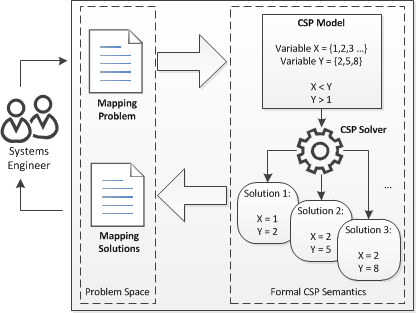
\includegraphics[width=.5\textwidth]{assist-process}
  \caption{Process to automatically construct a solution for a mapping problem}
  \label{fig:assist-process}
\end{figure}

\subsection{Toolsuite ASSIST}

As a proof of concept, the toolsuite \emph{Architecture Synthesis for Safety-Critical Systems (ASSIST)}~\cite{ASSIST} was developed by the authors.
It is open source and uses the constraint solver \emph{Choco}~\cite{Prudhomme2016} internally.
ASSIST (see Figure~\ref{tool}) allows a systems engineer to automatically construct and optimize mappings based on textual specifications of the
\begin{itemize}
\item mappable elements,
\item (safety) constraints for valid/invalid assignments and 
\item optimization goals.
\end{itemize}
The textual specifications in ASSIST conform to a domain-specific language which was jointly developed with the partners in the projects.
This approach allows to hide the intricacies of a formal specification.
Using a domain-specific language is expedient to enable systems engineers without a formal education in computer science to specify a mapping problem.

\begin{figure}[!t]
\centering
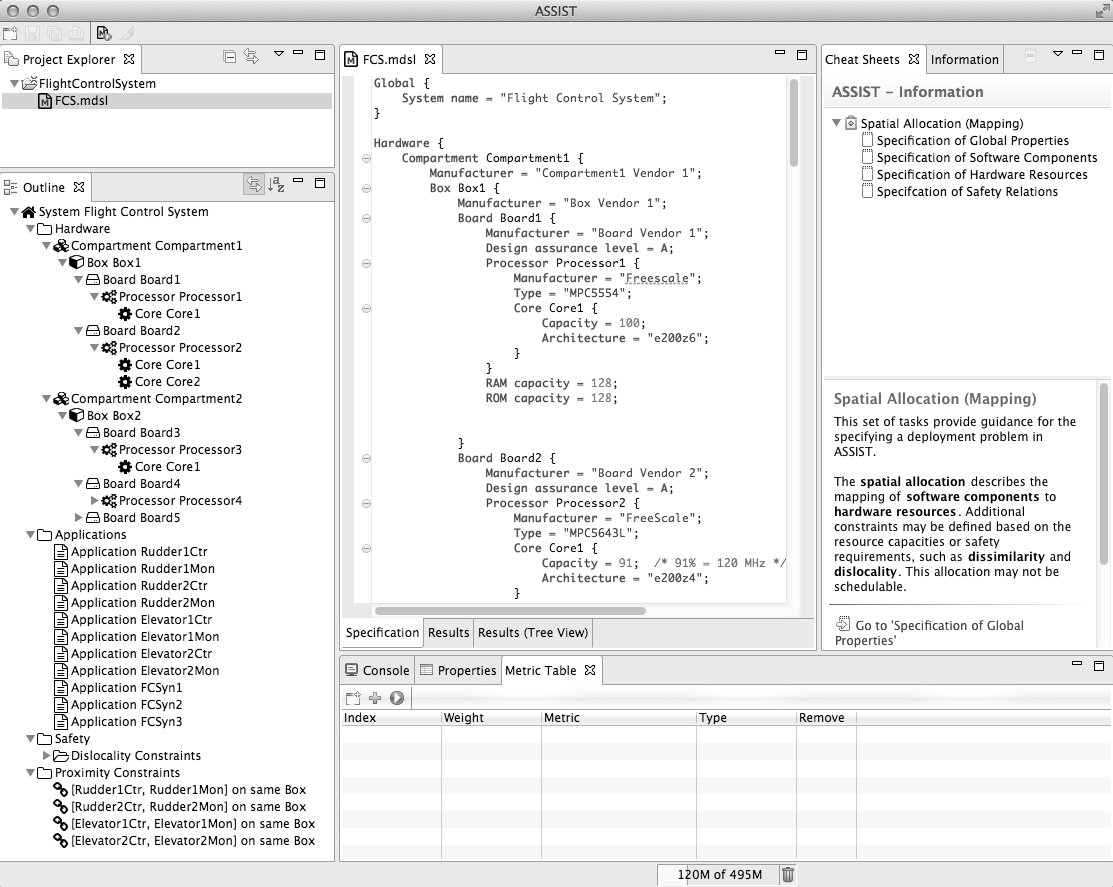
\includegraphics[height=7cm]{tool}
\caption{Screenshot of ASSIST with a specification for a control system}
\label{tool}
\end{figure}


\section{Ensuring Redundancy by Requiring Dislocality}

\begin{itemize}
\item In order to ensure a reliability / redundancy work properly - it is essential to ensure is differences
\item Differences in the deployment of redundant software components to make sure that the errors do not appear in the same manner at the same location (zonal effects)
\item Dislocality is a typical constraint in ASSIST to express these differences
\item Simple Modeling approach for a CSP (location variables)
\item Use allDiffererent constraint - straight forward
\end{itemize}

\printbibliography[heading=bibintoc]

\end{document}

%%% Local Variables: 
%%% mode: latex
%%% ispell-check-comments: exclusive
%%% ispell-local-dictionary: "english"
%%% End:
